\section{Result and Analysis}\label{sec:result_and_analysis}

\subsection{Dataset}\label{subsec:dataset}

% To test the selection system, we used three datasets. All three datasets have very different structures. Dataset 1 [\citenum{sakar2019comparative,parkinsons_disease_classification}] contains 149 records with 23 features. Dataset 2 [\citenum{little2007exploiting,parkinsons_disease_detection}] contains 201 records with 754 features. Dataset 3 [\citenum{ecg_heartbeat}] contains 65661 records with 188 features.

% To test the selection system, we used three datasets. All three datasets have very different structures. Dataset 1 contains 149 records with 23 features [\citenum{parkinsons_disease_classification}]. Dataset 2 contains 201 records with 754 features [\citenum{parkinsons_disease_detection}]. Dataset 3 contains 65661 records with 188 features [\citenum{ecg_heartbeat}].

To test the selection system, we used three datasets. All three datasets have very different structures. Dataset 1 contains 149 records with 23 features [\citenum{parkinsons_disease_classification}]. Dataset 2 contains 201 records with 754 features [\citenum{parkinsons_disease_detection}]. Dataset 3 contains 65661 records with 188 features [\citenum{ecg_heartbeat}].

Dataset 1 is the smallest dataset with a lower number of features compared to other two datasets. Dataset 2 also contains few records, but contains the highest amount of features compared to other two datasets. While, dataset 3 has a large number of records and moderate amount of features.

\subsection{Results}\label{subsec:results}

After providing the datasets mentioned in the previous section, the system trained a few models on those datasets. The application selected the best-suited model based on datasets. 

\autoref{fig:performance_analysis_dataset_1}, shows the performance of various models trained on dataset 1. Due to the small number of records and few features model is overtrained in the case of few models. The values in \autoref{tab:performance_analysis_dataset_1}, suggest that KNN and RF models were overtrained. The KNN model is selected as the best model for this dataset.

\begin{figure}[ht]
    \centering
    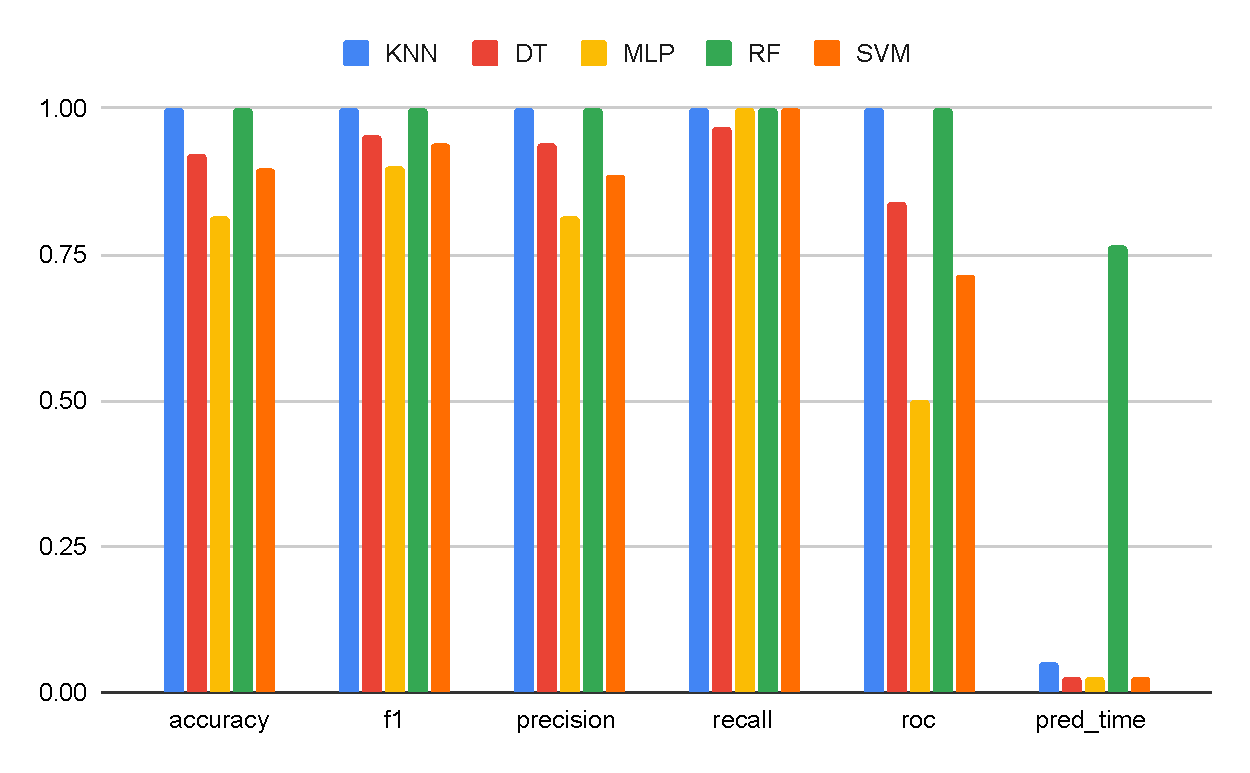
\includegraphics[width=0.9\columnwidth]{media/sec04/dataset_1_performance_evaluation.pdf}
    \caption{Performance Analysis Dataset 1}
    \label{fig:performance_analysis_dataset_1}
\end{figure}

\begin{table}[ht]
\caption{Performance Analysis of Dataset 1}\label{tab:performance_analysis_dataset_1}
\begin{tabular*}{\tblwidth}{@{}LLLLLL@{}}
\toprule
Metrics & KNN & DT & MLP & RF & SVM \\ % Table header row
\midrule
Accuracy & 1.00 & 0.92 & 0.82 & 1.00 & 0.89 \\
F1 & 1.00 & 0.95 & 0.89 & 1.00 & 0.94 \\
Pricision & 1.00 & 0.93 & 0.82 & 1.00 & 0.88 \\
Recall & 1.00 & 0.97 & 1.00 & 1.00 & 1.00 \\
ROC & 1.00 & 0.84 & 0.50 & 1.00 & 0.71 \\
Time & 0.05 & 0.02 & 0.02 & 0.76 & 0.02 \\
\bottomrule
\end{tabular*}
\end{table}

\autoref{fig:performance_analysis_dataset_2}, shows the performance of various models trained on dataset 2. This dataset also had a small number of records, but the number of features is extremely high. The values from \autoref{tab:performance_analysis_dataset_2}, shows the random forest performed better across all parameters but prediction time. The system selected the Random Forest model as best suited mode.

\begin{figure}[ht]
    \centering
    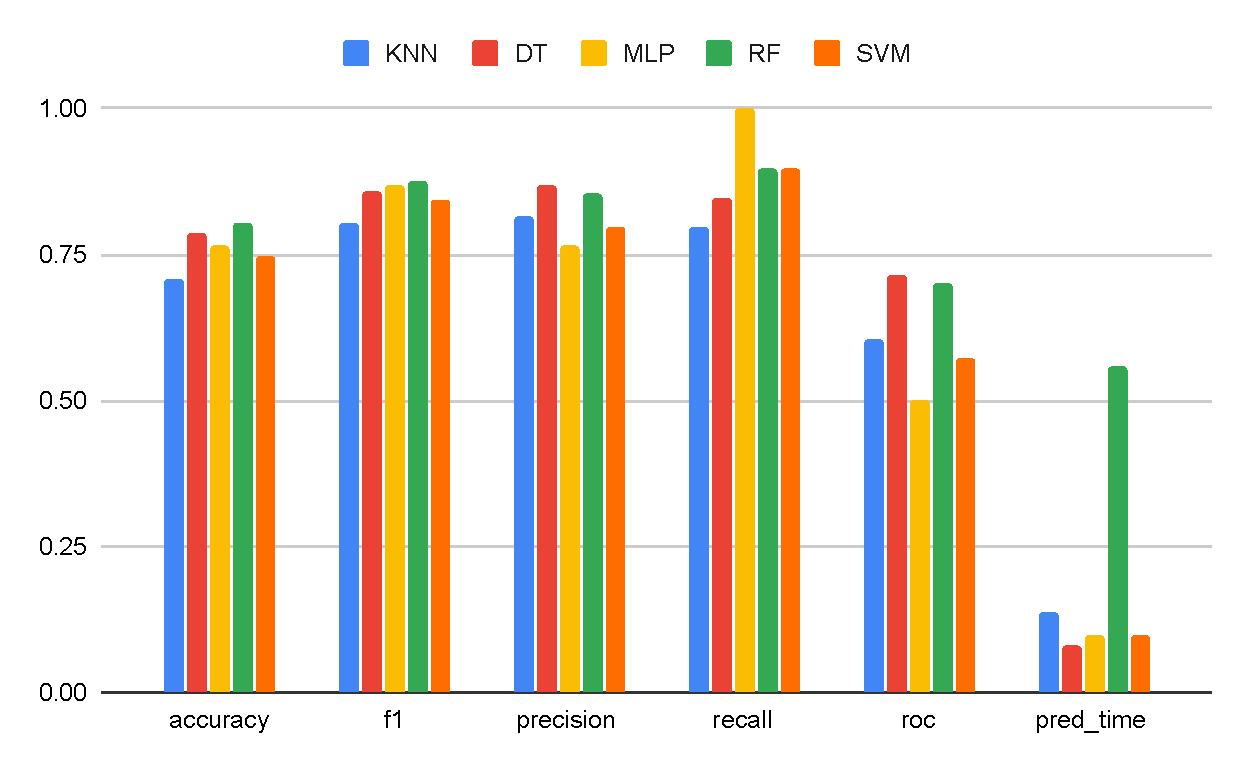
\includegraphics[width=0.9\columnwidth]{media/sec04/dataset_2_performance_evaluation.pdf}
    \caption{Performance Analysis Dataset 2}
    \label{fig:performance_analysis_dataset_2}
\end{figure}

\begin{table}[ht]
\caption{Performance Analysis of Dataset 2}\label{tab:performance_analysis_dataset_2}
\begin{tabular*}{\tblwidth}{@{}LLLLLL@{}}
\toprule
Metrics & KNN & DT & MLP & RF & SVM \\ % Table header row
\midrule
Accuracy & 0.71 & 0.78 & 0.76 & 0.80 & 0.75 \\
F1 & 0.81 & 0.86 & 0.87 & 0.88 & 0.84 \\
Precision & 0.82 & 0.67 & 0.76 & 0.85 & 0.80 \\
Recall & 0.79 & 0.85 & 1.00 & 0.90 & 0.90 \\
ROC & 0.61 & 0.71 & 0.50 & 0.70 & 0.57 \\
Time & 0.13 & 0.07 & 0.09 & 0.55 & 0.09 \\
\bottomrule
\end{tabular*}
\end{table}

\autoref{fig:performance_analysis_dataset_3}, shows the performance of various models trained on dataset 3. This dataset had a very high number of records and a moderate amount of features. The values from \autoref{fig:performance_analysis_dataset_3}, shows that almost all models performed satisfactorily on this dataset. The system selected the SVM model as best suited mode.

\begin{figure}[ht]
    \centering
    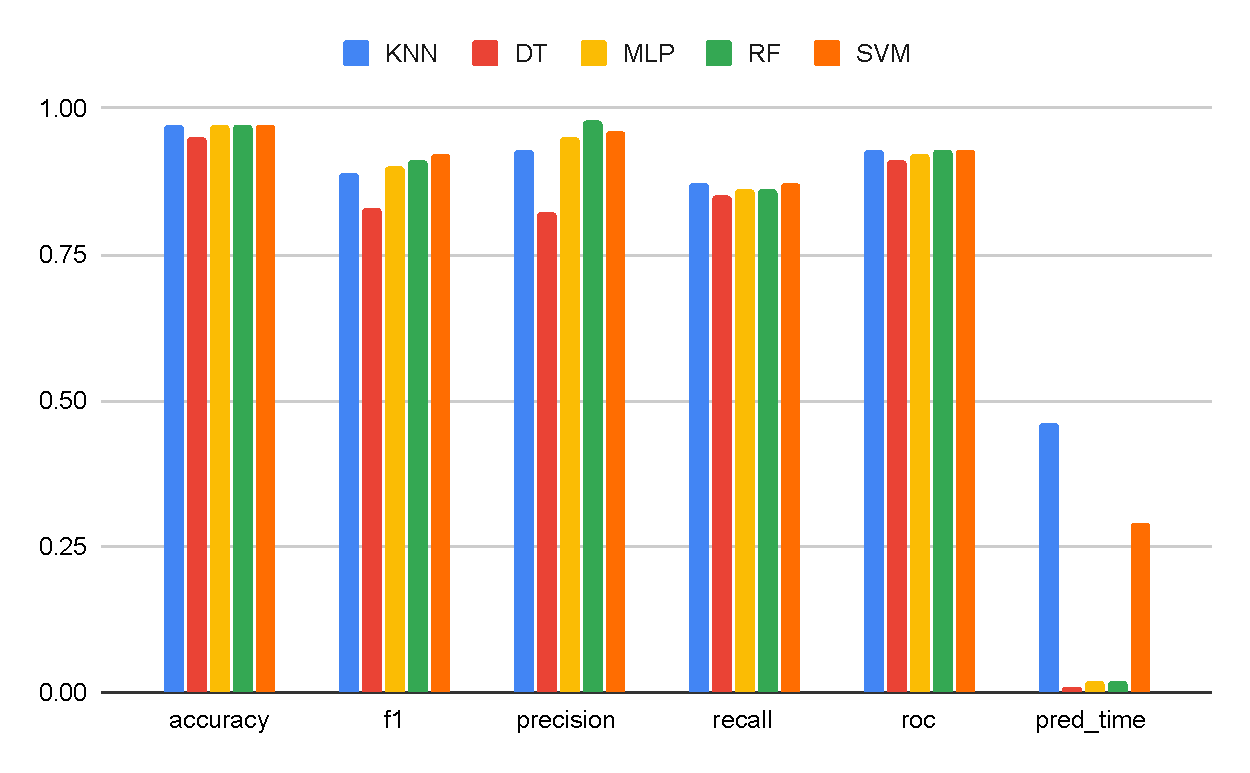
\includegraphics[width=0.9\columnwidth]{media/sec04/dataset_3_performance_evaluation.pdf}
    \caption{Performance Analysis Dataset 3}
    \label{fig:performance_analysis_dataset_3}
\end{figure}

\begin{table}[ht]
\caption{Performance Analysis of Dataset 3}\label{tab:performance_analysis_dataset_3}
\begin{tabular*}{\tblwidth}{@{}LLLLLL@{}}
\toprule
Metrics & KNN & DT & MLP & RF & SVM \\ % Table header row
\midrule
Accuracy & 0.97 & 0.95 & 0.97 & 0.97 & 0.97 \\
F1 & 0.89 & 0.83 & 0.90 & 0.91 & 0.92 \\
Precision & 0.93 & 0.82 & 0.95 & 0.98 & 0.96 \\
Recall & 0.87 & 0.85 & 0.86 & 0.86 & 0.87 \\
ROC & 0.93 & 0.91 & 0.92 & 0.93 & 0.93 \\
Time & 0.46 & 0.01 & 0.02 & 0.02 & 0.29 \\
\bottomrule
\end{tabular*}
\end{table}

\subsection{Key Findings}\label{subsec:key_findings}
From the data displayed in previous section, we saw how the system works on different datasets. These are a few key findings we obtained from that knowledge.
\begin{enumerate}
    \item The system successfully works on different scales of data.
    \item Systems performance does not depends on the number of records.
    \item Systems performance is dependent on the number of features of a dataset.
    \item The system is prone to overfitting depending on the scale of the dataset. Specifically, KNN and RF models tend to overfit with the small scale of data.
    \item The system successfully uses the tuning parameters to select the most suited model from the dataset.
\end{enumerate}

\subsection{Benefits of the System}\label{subsec:benefits_of_system}

The system can be used for any scale of data. It allows users with limited prior knowledge easier access to machine learning technology. As seen in previous section, the system can train multiple models effectively.

The user-defined fine-tuning parameters lead to the selection of the best-suited model for particular tasks. This model can be used to generate predictions in the case of similar datasets. The performance of all models is stored for future evaluation of the system.

\subsection{Improvements On the System}\label{subsec:improvements_on_system}

Currently, the system is limited to only five machine learning algorithms. With the smaller scale of data, specifically with a small number of features, the system tends to overfit the models.  Allowing users to implement their model templates will solve both of these problems.

These algorithms are supervised learning algorithms. The supervised nature of these algorithms limits the training dataset to the labeled dataset. By providing support to unsupervised learning algorithms, systems can accommodate various types of training datasets.

The selection parameters are adjusted before the training process. These predefined parameters restrict the selection choices of the system. Allowing users to tweak selection parameters can increase systems choices.
